% 2012_chongqing_science_q19_fig1: right triangular prism ABC-A1B1C1, D on AB (schematic)
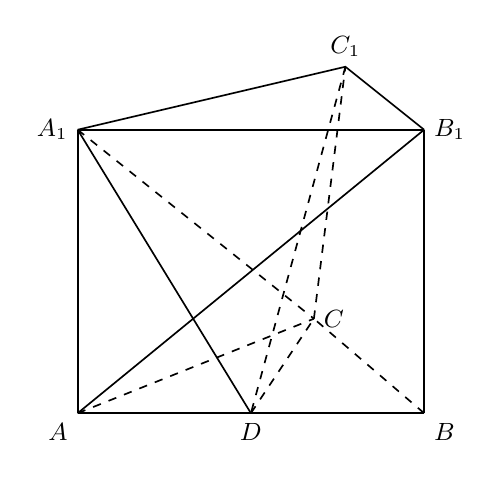
\begin{tikzpicture}[line width=0.6pt, font=\small]
\coordinate (A) at (0,0);
\coordinate (D) at (2.2,0);
\coordinate (B) at (4.4,0);
\coordinate (A1) at (0,3.6);
\coordinate (B1) at (4.4,3.6);
\coordinate (C) at (3.0,1.2);
\coordinate (C1) at (3.4,4.4);
% solid visible
\draw (A) -- (D) -- (B);
\draw (A) -- (A1);
\draw (B) -- (B1);
\draw (A1) -- (B1);
\draw (A1) -- (C1) -- (B1);
\draw (A) -- (B1);
\draw (A1) -- (D);
% dashed hidden
\draw[dashed] (A) -- (C);
\draw[dashed] (B) -- (C);
\draw[dashed] (D) -- (C);
\draw[dashed] (C) -- (C1);
\draw[dashed] (A1) -- (C);
\draw[dashed] (C1) -- (D);
\node[below left] at (A) {$A$};
\node[below] at (D) {$D$};
\node[below right] at (B) {$B$};
\node[left] at (A1) {$A_{1}$};
\node[right] at (B1) {$B_{1}$};
\node[right] at (C) {$C$};
\node[above] at (C1) {$C_{1}$};
\end{tikzpicture}
